\section{Applications of VAM to quantum and nuclear processes}
\label{sec:LENR_QED}
\subsection*{LENR via resonance tunneling}

Gravitational decay due to vorticity temporarily lowers the Coulomb barrier:

\begin{equation}
    V_\text{Coulomb} = \frac{Z_1 Z_2 e^2}{4\pi \varepsilon_0 r}, \quad \Delta P = \frac{1}{2} \rho_\text{\ae} r_c^2 (\Omega_1^2 + \Omega_2^2)
\end{equation}

Resonance occurs when:

\begin{equation}
    \Delta P \geq \frac{Z_1 Z_2 e^2}{4\pi \varepsilon_0 r_t^2}
\end{equation}

Rather than invoking purely probabilistic tunneling, VAM attributes the transition to real pressure gradients in a structured æther, paralleling the causal flow picture of Holland~\cite{holland1993quantum}

\subsection*{Resonant Ætheric tunneling and LENR in VAM}

In the Vortex Æther Model (VAM), low-energy nuclear reactions (LENR) are reinterpreted as resonant tunneling events mediated by structured vortex interactions in the Æther. Unlike conventional quantum tunneling, which relies on particle wave functions penetrating a static Coulomb potential barrier, VAM posits that local pressure minima – arising from vortex-induced Bernoulli deficits – can temporarily reduce or completely eliminate the barrier~\cite{Barcelo2011,volovik2003}.

The classical Coulomb repulsion between two nuclei of charges \( Z_1 e \) and \( Z_2 e \) is given by:
\begin{equation}
    V_\text{Coulomb}(r) = \frac{Z_1 Z_2 e^2}{4\pi \varepsilon_0 r}
\end{equation}

In VAM, two rotating vortex nodes in the vicinity of \( r \sim 2r_c \) generate a vortex-induced pressure drop~\cite{Saffman1992} via:
\begin{equation}
    \Delta P = \frac{1}{2} \rho_\text{\ae} r_c^2 (\Omega_1^2 + \Omega_2^2)
\end{equation}

This pressure drop changes the effective interaction potential:
\begin{equation}
    V_\text{eff}(r) = V_\text{Coulomb}(r) - \Phi_\omega(r)
\end{equation}
where the eddy potential \( \Phi_\omega(r) \) is defined by:
\begin{equation}
    \Phi_\omega(r) = \gamma \int \frac{|\vec{\omega}(r')|^2}{|\vec{r} - \vec{r}'|} \, d^3r',
    \quad \text{with} \quad
    \gamma = G \rho_\text{\ae}^2
\end{equation}

Resonant tunneling occurs when the combined effect of \( \Delta P \) and \( \Phi_\omega \) neutralizes the Coulomb barrier at a critical separation \( r_t \):
\begin{equation}
    \frac{1}{2} \rho_\text{\ae} r_c^2 (\Omega_1^2 + \Omega_2^2) \geq \frac{Z_1 Z_2 e^2}{4\pi \varepsilon_0 r_t^2}
\end{equation}

The resulting condition allows for transitions even at thermal or subthermal kinetic energies, allowing LENR processes to occur without actually having to overcome the barrier. Instead, it is dynamically erased via eddy resonance – a mechanism consistent with some empirical observations~\cite{Storms2021}. The tunneling is thus a manifestation of ætheric phase alignment and pressure-mediated coherence in confined vortex configurations.

\subsection*{VAM Quantum Electrodynamics (QED) Lagrangian}

In the Vortex Æther Model (VAM), the interaction between vortex nodes and electromagnetic fields arises from their helical structure and the associated induced vector potentials. The standard Lagrangian of quantum electrodynamics (QED) is replaced in this model by:

\begin{equation}
    \mathcal{L}_\text{VAM-QED} =
    \bar{\psi} \left[ i \gamma^\mu \partial_\mu
                   - \gamma^\mu \left( \frac{C_e^2 r_c}{\lambda_c} \right) A_\mu
                   - \left( \frac{8\pi \rho_\text{\ae} r_c^3 Lk}{C_e} \right) \right] \psi
    - \frac{1}{4} F_{\mu\nu} F^{\mu\nu}
\end{equation}

In this formulation:

\begin{itemize}
    \item Does the mass arise as a result of topological connected vortex cores, where the helicity of the vortex structure plays the role of mass~\cite{volovik2003}.
    \item The gauge coupling arises from æther circulation and the resulting vector potential.
    \item The electromagnetic field tensor \( F_{\mu\nu} \) remains unchanged, which describes the rotation of the æther (the curl component) in the surrounding superfluid.
\end{itemize}

This alternative Lagrangian thus directly couples vortex structures to field interactions, where the usual constants \( m \) (mass) and \( q \) (charge) are replaced by emergent terms arising from the geometry, rotation rate and topology of the æther medium.

By deriving the Euler–Lagrange equation for the spinor field \( \psi \), we find:

\begin{equation}
    \boxed{ \left( i \gamma^\mu \partial_\mu - \gamma^\mu q_\text{vortex} A_\mu - M_\text{vortex} \right)\psi = 0 }
\end{equation}

This equation is structurally identical to the Dirac equation, but with physical parameters arising from vortex mechanics instead of as fundamental data. Thus, VAM provides an alternative for the origin of mass and charge~\cite{Barcelo2011,volovik2003}.

\begin{figure}[H]
    \centering
    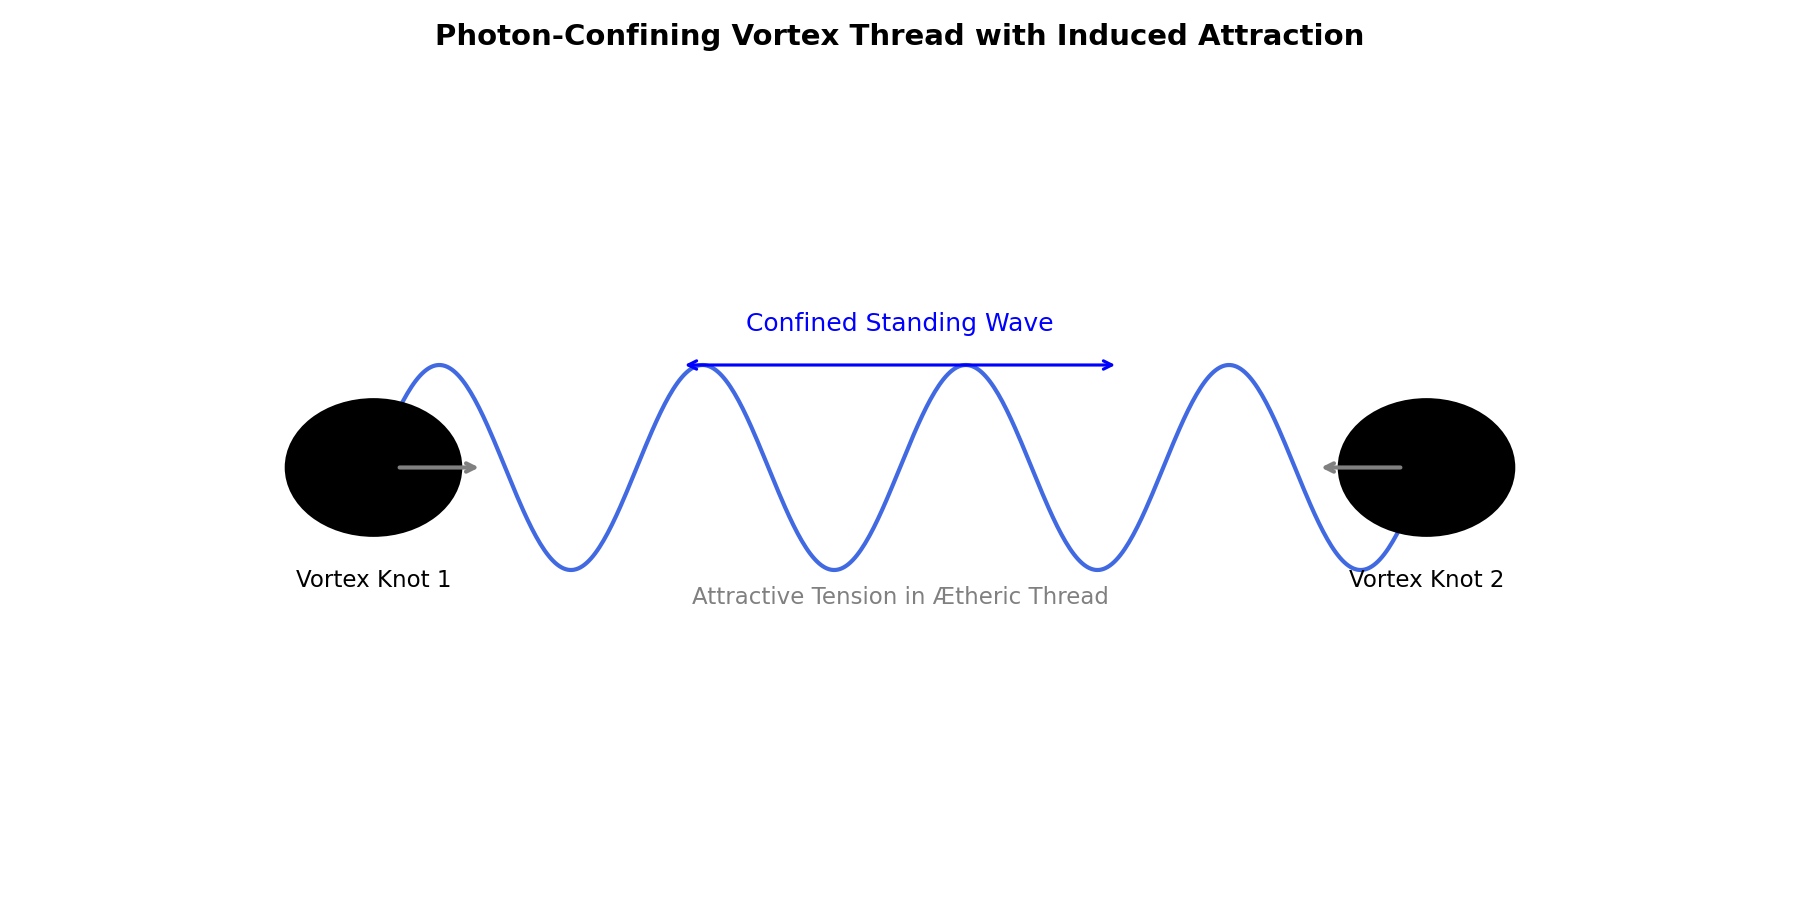
\includegraphics[width=0.85\textwidth]{images/08-Photon-ConfiningVortexThreadGravitation}
    \caption{Photon confinement and guidance along vortex threads in the æther. This visualizes the VAM interpretation of electromagnetic propagation, where the photon exhibits localized trajectory bending and resonance around structured vortex lines. The confinement arises naturally from topological pressure minima and circulating æther flow, replacing the abstract field representation with a tangible vortex-based channel.}
    \label{fig:photon_confine}
\end{figure}

\subsection{Emergent Bohr Radius from Vortex Swirl Pressure}
As a demonstration of how quantum orbitals emerge in VAM from core swirl parameters \((r_c, C_e)\), we derive the Bohr radius using force balance between æther tension and induced swirl pressure.

\subsection*{Standard Quantum Bohr Radius}
In canonical quantum mechanics, the Bohr radius is defined as:
\begin{equation}
    a_0 = \frac{4\pi \varepsilon_0 \hbar^2}{m_e e^2}
\end{equation}
This expression balances the centripetal force and Coulomb attraction in the hydrogen atom.

\subsection*{Swirl-Based Dynamics in VAM}
In VAM, the electron is a topological knotted vortex. The swirl velocity induced at a radial distance \( r \) is:
\begin{equation}
    v_\phi(r) = \frac{\Gamma}{2\pi r}, \quad \text{where } \Gamma = 2\pi r_c C_e
\end{equation}
So:
\begin{equation}
    v_\phi(r) = \frac{r_c C_e}{r}
\end{equation}

\subsection*{Force Balance}
Balancing centrifugal and Coulomb-like force:
\begin{equation}
    \frac{m_e v_\phi^2(r)}{r} = \frac{e^2}{4\pi \varepsilon_0 r^2}
\end{equation}
Substituting \( v_\phi(r) = \frac{r_c C_e}{r} \):
\begin{equation}
    \frac{m_e (r_c C_e)^2}{r^3} = \frac{e^2}{4\pi \varepsilon_0 r^2}
\end{equation}
Multiply both sides by \( r^3 \):
\begin{equation}
    m_e r_c^2 C_e^2 = \frac{e^2 r}{4\pi \varepsilon_0}
\end{equation}
Solve for \( r = a_0 \):
\begin{equation}
    \boxed{a_0 = \frac{4\pi \varepsilon_0 m_e r_c^2 C_e^2}{e^2}}
\end{equation}

\subsection*{Numerical Evaluation}
Using:
\begin{align*}
    \varepsilon_0 &= 8.854187817 \times 10^{-12}~\si{F/m} \\
    m_e &= 9.1093837015 \times 10^{-31}~\si{kg} \\
    r_c &= 1.40897017 \times 10^{-15}~\si{m} \\
    C_e &= 1.09384563 \times 10^6~\si{m/s} \\
    e &= 1.602176634 \times 10^{-19}~\si{C}
\end{align*}
Substitute into Eq. (7):
\begin{equation}
    a_0 \approx 5.29 \times 10^{-11}~\si{m}
\end{equation}
\noindent
which matches the canonical Bohr radius.

\subsection*{Interpretation}
In VAM, the Bohr radius \( a_0 \) is where the vortex swirl pressure gradient balances ætheric tension. This corresponds to the radius of stable resonance in the induced swirl field:
\begin{equation}
    \boxed{\text{Bohr radius} = \text{tidal resonance of knotted vortex pressure field}}
\end{equation}
This pressure-based derivation echoes early causal interpretations of quantum mechanics, where the particle trajectory is guided by structured wave-like fields rather than probabilistic axioms~\cite{holland1993quantum}

\subsection*{Future Work}
This framework allows derivation of hydrogenic energy levels and fine structure constants using vortex core parameters \( r_c, C_e \), and æther density \( \rho_\ae \).
